\section{Filtro 3: HSL}

\subsection{Explicacion}

La idea de este filtro consiste en transformar una imagen del espacio RGB a HSL, sumarle un valor recibido por parametro a cada una de las componentes y luego convertir la imagen de HSL a RGB, esto debe hacerse sobre la totalidad de los pixeles. Para las conversiones de espacio y la suma, la catedra proveyo las ecuaciones apropiadas junto con una implementacion en $C$ de las tres etapas.

\subsection{Implementacion 1}

Para la primer implementacion habia que implementar unicamente la etapa de $suma$ en $Assembler$, utilizando las funciones de $C$ provistas por la catedra para la conversion de RGB a HSL y viceversa. La ecuaciones de $suma$ son las siguientes:

\begin{align*}
suma_h(h, HH) =
\begin{cases}
h + HH - 360 &\mbox{si}\ h + HH \geq 360\\
h + HH + 360 &\mbox{si}\ h + HH < 0     \\
h + HH
\end{cases}
\\
suma_s(s, SS) =
\begin{cases}
1 &\mbox{si}\ s + SS \geq 1\hspace{17mm}\\
0 &\mbox{si}\ s + SS < 0   \\
s + SS
\end{cases}
\\
suma_l(l, LL) =
\begin{cases}
1 &\mbox{si}\ l + LL \geq 1\hspace{18mm}\\
0 &\mbox{si}\ l + LL < 0   \\
l + LL
\end{cases}
\end{align*}

Para las operaciones con punto flotante se empleo el tipo $float$. Para comenzar las operaciones de $suma$, partimos de los siguientes registros \texttt{XMM} con sus respectivos valores:\\

\noindent
\texttt{XMM0 $\gets$   LL  $\vert$   SS  $\vert$   HH  $\vert$ - }\\
\texttt{XMM1 $\gets\ $   l  $\vert\ $   s  $\vert\ $   h  $\vert$ - }\\

Tambien se cargaron en las siguientes mascaras:\\

\noindent
\texttt{XMM2 $\gets$  1.0  $\vert$  1.0  $\vert\ $  0.0  $\ \vert$ - }\\
\texttt{XMM3 $\gets$  0.0  $\vert$  0.0  $\vert\ $  0.0  $\ \vert$ - }\\
\texttt{XMM6 $\gets$  0.0  $\vert$  0.0  $\vert$  360.0  $\vert$ - }\\
\texttt{XMM7 $\gets$  0.0  $\vert$  0.0  $\vert\ $  0.0  $\ \vert$ - }\\
\texttt{XMM8 $\gets$  0.0  $\vert$  0.0  $\vert$  360.0  $\vert$ - }\\
\texttt{XMM9 $\gets$  0.0  $\vert$  0.0  $\vert$  360.0  $\vert$ - }\\

Con estos valores en los registros, se procedio a realizar la suma de la componentes de \texttt{XMM0} y \texttt{XMM1} con la instruccion \texttt{ADDPS} guardando el resultado en \texttt{XMM0}, y luego se almcenaron dos copias del mismo en \texttt{XMM4} y \texttt{XMM5} mediante la instruccion \texttt{MOVDQU}

La copia de \texttt{XMM4} se utilizo junto con las mascaras \texttt{XMM2} y \texttt{XMM3}, para poder satisfacer $suma_s$ y $suma_l$. Primero se tomo el minimo entre \texttt{XMM4} y \texttt{XMM2}, almacenando el resultado en \texttt{XMM4}, luego se procedio a tomar el maximo entre \texttt{XMM4} y \texttt{XMM3}, nuevamente guardando el resultado en \texttt{XMM4}. Esto nos sirve para respetar la funcion de $suma_s$ y $suma_l$, ya que en caso de que nuestros valores de $s$ o $l$ se excedan de \texttt{1.0}, el mismo pasaria a ser \texttt{1.0}, el mismo razonamiento aplica en el caso de que alguna de esas dos componentes sea menor a \texttt{0.0}.
\newpage
Una vez que tenemos los valores correspondientes en \texttt{XMM4}, procedemos a hacer un shuffle con el registro XMM0. El mismo lo hacemos con la instruccion \textsc{SHUFPS}, este responde al comportamiento mostrado en el siguiente grafico:

\begin{figure}[!h]
	\centering
	\includegraphics[scale=1.25]{images/HSLASM1_0}
\end{figure}

Con los valores correctos de $s + SS$ y $l + LL$, solo queda analizar $h + HH$. Para hacer esto empleamos las mascaras de \texttt{XMM6} y \texttt{XMM7}, procedimos a hacer una comparacion entre estas y el registro \texttt{XMM5} para obtener las nuevas mascaras que nos permitieron filtrar los condicionales de $suma_h$. La secuencia de operaciones fue la siguiente:\\

\noindent
\texttt{XMM6 $\gets$ XMM5 $\geq$ 360.0} \\
\texttt{XMM7 $\gets$ XMM5 $\geq$ 0} \\
\texttt{XMM6 $\gets$ XMM5 AND XMM8} \\
\texttt{XMM7 $\gets$ NOT(XMM7) AND XMM9} \\

Para las comparaciones se utilizo \texttt{CMPPS} y para las ultimas dos se utilizo \texttt{ANDPS} y \textsc{ANDNPS} respectivamente. Una vez finalizadas estas operaciones, si $h + HH$ se excede o iguala a \texttt{360.0}, en el tercer float de \texttt{XMM6} tendriamos el valor \texttt{360.0} mientras que en el caso que $h + HH$ sea menor a \texttt{0.0}, tendriamos el valor \texttt{360.0} en el tercer float de \texttt{XMM7}, si no se cumplen esas condiciones tendriamos el valor \texttt{0.0} en el tercer float del registro que no haya cumplido con el condicional. Con estos valores, lo unica operacion faltante fue a \texttt{XMM0} restarle \texttt{XMM6}, a este luego sumarle \texttt{XMM7} y guardar el resultado en \texttt{XMM0}, esto nos permite satisfacer el condicional de $suma_h$, y como originalmente \texttt{XMM6} y \texttt{XMM7} tenia \texttt{0.0} en los primeros dos $float$, esto hace que la ultima suma y resta no afecte los valores de $s$ y $l$, ya que tanto \texttt{XMM6} y \texttt{XMM7} siguen teniendo \texttt{0.0} en los primeros dos $float$. Teniendo en cuenta esto, tenemos finalmente en \texttt{XMM0} un registro que cumple con:\\

\noindent
\texttt{XMM0 $\gets$} $suma_l(l,LL)$ $\vert$ $suma_s(s,SS)$ $\vert$ $suma_h(h,HH)$ $\vert$ - \\

Con esto concluimos la etapa $suma$ de la primer implementacion, solo resta llamar a la funcion $HSLtoRGB$ provista por la catedra y volcar el resultado de la conversion en memoria.

\subsection{Implementacion 2}

Para la segunda implementacion se nos pidio implementar las 3 etapas del filtro en $Assembler$. Para la etapa $suma$ se utilizo la misma implementacion que la primera.

\subsubsection{RGB a HSL}

Al igual que el caso de $suma$, la catedra proveyo de las ecuaciones apropiadas. Las mismas estan presentadas a continuacion:

\begin{align*}
h(r, g, b) =
\begin{cases}
0 &\mbox{si}\ cmax = cmin\\
60* (g-b)/d + 6 &\mbox{si}\ cmax = r \\
60* (b-r)/d + 2 &\mbox{si}\ cmax = g \\
60* (r-g)/d + 4 &\mbox{si}\ cmax = b 
\end{cases}
\pmod{360}\hspace{17mm}
\\
l(r, g, b) = \frac{cmax + cmin}{510}\hspace{73mm}
\\
s(r, g, b) =
\begin{cases}
0 &\mbox{si}\ cmax = cmin \\
(d/(1-\texttt{fabs}(2*l(r, g, b) - 1)))/255.0001
\end{cases}
\end{align*}

Donde $cmax = max(r,g,b)$, $cmin = min(r,g,b)$ y $d = cmax - cmin$.

\paragraph{Calculo de \texttt{h}\newline}

Primero procedimos a levantar las componentes del pixel de la memoria y copiarlo al registro \texttt{XMM1}, dicha operacion la hicimos con la instruccion \texttt{MOVD}. Despues desempaquetamos los datos de tipo $uint8$ a $int$, esto fue hecho mediante \texttt{PUNPCKLBW} y \texttt{PUNPCKLWD} en ese orden, aplicando las instruccion sobre \texttt{XMM1} junto con algun registro \texttt{XMM} que contenga \texttt{0} en todos sus bits. Una vez con los valores en su tamaño correspondiente, procedimos a calcular \texttt{cmax} y \texttt{cmin}, esto lo logramos utilizando tres copias de \texttt{XMM1}, aplicando shifts a dos de ellas y tomando el minimo y maximo vertical almacenando el resultado en \texttt{XMM5} y \texttt{XMM6} respectivamente, los shifts fueron logrados mediante las instrucciones \texttt{PSRLDQ} y \texttt{PSLLDQ} segun el sentido en el cual deseemos shiftear. Hasta este momento tenemos en los registros:\\

\noindent
\texttt{XMM0 $\gets\ $ B $\ \ \vert$ G $\vert$ R $\vert$ A}\\
\texttt{XMM1 $\gets\ $ B $\ \ \vert$ G $\vert$ R $\vert$ 0}\\
\texttt{XMM5 $\gets$ cmin    $\vert$ - $\vert$ - $\vert$ -}\\
\texttt{XMM6 $\gets$ cmax    $\vert$ - $\vert$ - $\vert$ -}\\

El registro \texttt{XMM0} contiene una copia con el canal $alpha$ preservado, esta sera utilizada unicamente al final de la conversion.
Con \texttt{cmin} y \texttt{cmax} en sus respectivos registros, procedimos a limpiarlos con una mascara y a hacer un shuffle con \texttt{XMM6}, copiando la componente \texttt{cmax} en las cuatro componentes de \texttt{XMM2}. Luego, hicimos una nueva copia de \texttt{XMM1} en \texttt{XMM3} y mediante un shift y un \texttt{OR} con \texttt{XMM5}, logramos juntar las componentes \texttt{cmin}, \texttt{R}, \texttt{G} y \texttt{B} en un solo registro. Entonces tenemos:\\

\noindent
\texttt{XMM5 $\gets$ cmin $\vert\ $ 0 $\ \ \vert\ $ 0  $\ \ \vert\ $ 0}\\
\texttt{XMM6 $\gets$ cmax $\vert\ $ 0 $\ \ \vert\ $ 0  $\ \ \vert\ $ 0}\\
\texttt{XMM2 $\gets$ cmax $\vert$ cmax    $\vert$ cmax $\vert$ cmax}\\
\texttt{XMM3 $\gets$ cmin $\vert\ $ B $\ \ \vert\ $ G  $\ \ \vert\ $ R}\\

Los registros \texttt{XMM2} y \texttt{XMM3} fueron empleados para obtener la mascara para poder calcular la funcion $h(r,g,b)$. La misma fue obtenida utilizando la instruccion \texttt{PCMPEQD} entre \texttt{XMM3} y \texttt{XMM2}, almacenando el resultado de la comparacion de igualdad en \texttt{XMM3}. Una vez obtenida esta mascara, la misma fue reordenada via un shuffle, para seguir el mismo orden que el condicional de la implementacion $C$, el nuevo orden fue guardado en el registo \texttt{XMM4}. En esta etapa tenemos:\\

\noindent
\texttt{XMM3 $\gets$ cmin == cmax $\vert$ B == cmax $\vert$ G == cmax  $\vert\ \ \ $ R == cmax}\\
\texttt{XMM4 $\gets\ \ \ $ R == cmax $\vert$ G == cmax $\vert$ B == cmax  $\vert$ cmin == cmax}\\

Uno de los problemas encontrados durante la implementacion fueron los casos donde existian 2 o mas componentes que eran iguales a \texttt{cmax}, esto hacia que la mascara tuviese mas de una componente con \texttt{0xFFFFFFFF}, lo cual hacia que los resultados al filtrar fuesen incorrectos. Para solucionar esto propusimos armar una mascara, la cual tuviese \texttt{0xFFFFFFFF} en las componentes despues la primer componente distinta de cero de \texttt{XMM4}, lo unico necesario seria hacer \texttt{XOR} bit a bit entre la nueva mascara y \texttt{XMM4}. El grafico a continuacion ilustra la idea:

\begin{figure}[!h]
	\centering
	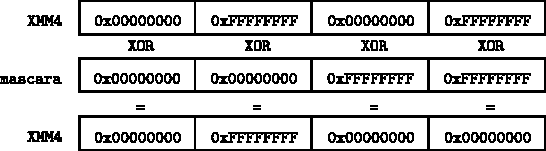
\includegraphics[scale=1.25]{images/HSLASM1_1}
\end{figure}

Una vez que tenemos esta mascara, preparamos los registros \texttt{XMM7}, \texttt{XMM8}, \texttt{XMM9} y \texttt{XMM11} con los siguientes valores y tambien disponiamos de una seria de constantes en memoria. Los valores de los registros y constantes son los siguientes:

\noindent
\texttt{XMM7  $\ \ \ \ \gets\ $ g $\ \ \vert\ $ b $\ \ \vert\ $ r  $\ \ \vert\ $ 0}\\
\texttt{XMM8  $\ \ \ \ \gets\ $ b $\ \ \vert\ $ r $\ \ \vert\ $ g  $\ \ \vert\ $ 0}\\
\texttt{XMM9  $\ \ \ \ \gets$ cmax $\vert$ cmax    $\vert$ cmax $\vert$ cmax}\\
\texttt{XMM11 $\ \ \ \gets$ cmin $\vert$ cmin    $\vert$ cmin $\vert$ cmin}\\
\texttt{cte\char`_suma $\gets\ $ 6.0 $\vert\ $ 2.0 $\vert\ $ 4.0 $\vert\ $ 0.0}\\
\texttt{cte\char`_60 $\ \ \gets$ 60.0 $\vert$ 60.0 $\vert$ 60.0 $\vert$ 60.0}\\

Se procedio a realizar las operaciones verticales apropiadas para poder satisfacer la funcion $h(r,g,b)$. La unica salvedad es que luego de efectuar las operaciones de resta entre \texttt{XMM7} y \texttt{XMM8}, y la de \texttt{XMM11} y \texttt{XMM9}, el resultado de ambas fue convertido a $float$ mediante la instruccion \texttt{CVTDQ2PS} y almcenado en los registros \texttt{XMM8} y \texttt{XMM10} respectivamente. Posteriormente se procedio con el resto de las operaciones con las instrucciones de punto flotante apropiadas, y se guardo el resultado en \texttt{XMM8}, a este luego se le aplico la mascara guardada en \texttt{XMM4}.

Otro problema que encontramos fue el caso \texttt{cmin == cmax}, aqui tenemos que \texttt{d} es igual a cero, con lo cual al proceder con las divisiones nos topariamos con un NaN, para solucionar esto decidimos armar una nueva mascara que contenga \texttt{cmin == cmax} en cada una de sus componentes. Para hacerlo alcanzo con utilizar el registro \texttt{XMM9} y \texttt{XMM2} (el mismo no fue modificado y mantiene los mismos valores que arriba) para hacer la comparacion de igualdad, el resultado de la misma fue guardado en \texttt{XMM9}. Con esto se procedio a hacer la operacion \texttt{NOT(XMM9) AND XMM8}, y para poder calcular el mód 360 de $h(r,g,b)$ se aplico la misma logica que en caso de $suma$ ya que los calculos para $h$ no van a excederse de 720. Finalmente tenemos en \texttt{XMM10}:\\

\noindent
\texttt{XMM10  $\gets$ - $\vert$ - $\vert$ - $\vert$ h}\\

\paragraph{Calculo de \texttt{l} y \texttt{s}\newline}

Para el calculo de \texttt{l} no hubo ninguna particularidad, el mismo se hizo en base a los siguientes registros y constantes:\\

\noindent
\texttt{XMM7 $\ \ \ \gets\ $ cmax $\vert\ \ $ 0 $\ \ \vert\ \ $ 0 $\ \ \vert\ \ $ 0}\\
\texttt{XMM5 $\ \ \ \gets\ $ cmin $\vert\ \ $ 0 $\ \ \vert\ \ $ 0 $\ \ \vert\ \ $ 0}\\
\texttt{cte\char`_510  $\gets$ 510.0 $\vert$ 510.0 $\vert$ 510.0 $\vert$ 510.0}\\

Primero se realizo la resta entre \texttt{XMM7} y \texttt{XMM5} almacenando el resultado en \texttt{XMM7}, a esta se la convirtio a $float$ mediante \texttt{CVTDQ2PS} previo a la multiplicacion con \texttt{cte\char`_510}. Tenemos finalmente en resultado en \texttt{XMM8}, el mismo tiene la pinta:\\

\noindent
\texttt{XMM8  $\gets$ l $\vert$ 0 $\vert$ 0 $\vert$ 0}\\

Para el calculo de \texttt{s} se utilizaron los siguientes registros, mascaras y constantes:\\

\noindent
\texttt{XMM7 $\ \ \ \ \ \ \ \gets\ \ \ $ cmax $\ \ \ \vert\ $ 0 $\ \vert\ $ 0 $\ \vert\ $ 0}\\
\texttt{XMM5 $\ \ \ \ \ \ \ \gets\ \ \ $ cmin $\ \ \ \vert\ $ 0 $\ \vert\ $ 0 $\ \vert\ $ 0}\\
\texttt{XMM5 $\ \ \ \ \ \ \ \gets\ \ \ \ $ l $\ \ \ \ \ \vert\ $ 0 $\ \vert\ $ 0 $\ \vert\ $ 0}\\
\texttt{cte\char`_1  $\ \ \ \ \ \ \gets\ \ \ $ 1.0 $\ \ \ \ \vert$ 1.0 $\vert$ 1.0 $\vert$ 1.0}\\
\texttt{cte\char`_2  $\ \ \ \ \ \ \gets\ \ \ $ 2.0 $\ \ \ \ \vert$ 2.0 $\vert$ 2.0 $\vert$ 2.0}\\
\texttt{cte\char`_255  $\ \ \ \ \gets\ $ 255.0001 $\ \vert\ $ 0 $\ \vert\ $ 0 $\ \vert\ $ 0}\\
\texttt{masc\char`_abs  $\ \ \ \gets$ 0x7FFFFFFF $\vert\ $ 0 $\ \vert\ $ 0 $\ \vert\ $ 0}\\
\texttt{limpiar\char`_msb  $\gets$ 0xFFFFFFFF $\vert\ $ 0 $\ \vert\ $ 0 $\ \vert\ $ 0}\\

En este caso hay dos puntos a destacar, estos son el condicional de $s(r,g,b)$ y el \texttt{fabs}. Para poder filtrar segun si \texttt{cmax == cmin} alcanza con hacer una comparacion de igualdad entre \texttt{cmax} y \texttt{cmin} mediante \texttt{PCMPEQD}, guardar el resultado de la misma en un registro, y luego de hacer las operaciones correspondientes aplicar el resultado de la comparacion mediante un \texttt{AND}. En el caso del \texttt{fabs}, al estar operando con numeros de tipo $float$ codificados bajo la norma IEEE 754, basta con colocar el bit mas significativo en cero, esto lo podemos hacer mediante un \texttt{AND} con el numero al cual deseamos aplicar \texttt{fabs} y la \texttt{masc\char`_abs}. Finalmente tenemos en el registro \texttt{XMM7}:\\

\noindent
\texttt{XMM7 $\gets$ s $\vert$ 0 $\vert$ 0 $\vert$ 0}\\

Con los valores de \texttt{h}, \texttt{s} y \texttt{l} calculados, lo unico que falta por hacer es juntar todo en un solo registro junto con el dato del canal $alpha$, el cual se encuentra en el registro \texttt{XMM0}. Para hacer esto, vamos a shiftear los registros que contienen a \texttt{s} y a \texttt{h}, 4 y 8 bytes hacia la derecha respectivamente. Una vez que tenemos esto, lo vamos a juntar a todos en un unico registro mediante un \texttt{OR} y vamos a procede a aplicarle a \texttt{XMM0} la mascara \texttt{limpiar\char`_msb}, convertir el resultado a $float$ y juntarlo junto con lo que ya teniamos utilizando nuevamente un \texttt{OR}. Con esto podemos concluir la etapa $RGBtoHSL$.

\subsubsection{HSL a RGB}

Tanto como en el caso de $suma$ y $RGBtoHSL$, la catedra proveyo las ecuaciones necesarias para la conversion, las mismas son:\\

\begin{align*}
RGBAux(h, s, l) =
\begin{cases}
(c,x,0) &\mbox{si}\ 0 \leq h < 60\\
(x,c,0) &\mbox{si}\ 60 \leq h < 120\\
(0,c,x) &\mbox{si}\ 120 \leq h < 180\\
(0,x,c) &\mbox{si}\ 180 \leq h < 240\\
(x,0,c) &\mbox{si}\ 240 \leq h < 300\\
(c,0,x) &\mbox{si}\ 300 \leq h < 360
\end{cases}
\hspace{62mm}
\\
RGB(h,s,l) = (RGBAux(h,s,l)_r * 255, RGBAux(h,s,l)_g * 255, RGBAux(h,s,l)_b * 255)
\end{align*}

Donde $c = (1 - fabs(2*l - 1))*s$, $x = c*(1 - fabs(fmod(h/60, 2) - 1))$ y $m = 1 - c/2$. Se tuvo que hacer un cambio, ya que en el enunciado las componentes \texttt{B} y \texttt{G} se encontraban invertidas, imposibilitando la conversion correcta.

Para poder hacer el calculo de \texttt{R}, \texttt{G}, \texttt{B} tuvimos que hacer el de \texttt{c}, \texttt{x} y \texttt{m}.

\paragraph{Calculo de \texttt{c}\newline}

Para el calculo de \texttt{c}, tenemos los siguientes registros, mascaras y constantes:\\

\noindent
\texttt{XMM1 $\ \ \ \ \gets \ \ \ \ $ l $\ \ \ \ \ \vert\ \ \ \ $ l $\ \ \ \ \ \vert\ \ \ \ $ l  $\ \ \ \ \ \vert\ \ \ \ $ l}\\
\texttt{XMMn $\ \ \ \ \gets \ \ \ \ $ s $\ \ \ \ \ \vert\ \ \ \ $ s $\ \ \ \ \ \vert\ \ \ \ $ s  $\ \ \ \ \ \vert\ \ \ \ $ s}\\
\texttt{cte\char`_1 $\ \ \ \gets\ \ \ $ 1.0 $\ \ \ \ \vert\ \ \ $ 1.0 $\ \ \ \ \vert\ \ \ $ 1.0 $\ \ \ \ \vert\ \ \ $ 1.0}\\
\texttt{cte\char`_2 $\ \ \ \gets\ \ \ $ 2.0 $\ \ \ \ \vert\ \ \ $ 2.0 $\ \ \ \ \vert\ \ \ $ 2.0 $\ \ \ \ \vert \ \ \ $ 2.0}\\
\texttt{masc\char`_abs $\gets$ 0x7FFFFFFF $\vert$ 0x7FFFFFFF $\vert$ 0x7FFFFFFF $\vert$ 0x7FFFFFFF}\\

Con estos podemos hacer las operaciones correspondientes para satisfacer el calculo de \texttt{c}. El unico caso que requiere atencion particular es el de \texttt{fabs}, debido a que los numeros de punto flotante estan codificados con la norma IEEE 754, lo unico que hace falta para poder obtener el valor absoluto es colocar el bit mas significativo de cada $float$ en cero, para hacer esto alcanza con aplicar la mascara \texttt{masc\char`_abs} mediante la instruccion \texttt{ANDPS} al registro apropiado. Tras finalizar las operaciones tenemos en \texttt{XMM1}:\\

\noindent
\texttt{XMM1 $\gets$ c $\vert$ c $\vert$ c $\vert$ c}\\

Posteriormente procedimos a limpiar el registro, dejando unicamente el $float$ de las posicion menos significativa. Entonces obtenemos:\\

\noindent
\texttt{XMM1 $\gets$ 0 $\vert$ 0 $\vert$ 0 $\vert$ c}\\

Esto lo hacemos para despues poder armar todas las posiblidades de $RGBAux(h,s,l)$.

\paragraph{Calculo de \texttt{x}\newline}

Al igual que con \texttt{c}, vamos a empezar por los registros:\\

\noindent
\texttt{XMM0 $\ \ \ \ \gets \ \ \ \ $ l $\ \ \ \ \ \vert\ \ \ \ $ s $\ \ \ \ \ \vert\ \ \ \ $ h  $\ \ \ \ \ \vert\ \ \ \ $ a}\\
\texttt{XMM1 $\ \ \ \ \gets \ \ \ \ $ 0 $\ \ \ \ \ \vert\ \ \ \ $ 0 $\ \ \ \ \ \vert\ \ \ \ $ 0  $\ \ \ \ \ \vert\ \ \ \ $ c}\\
\texttt{XMM3 $\ \ \ \ \gets \ \ \ \ $ h $\ \ \ \ \ \vert\ \ \ \ $ h $\ \ \ \ \ \vert\ \ \ \ $ h  $\ \ \ \ \ \vert\ \ \ \ $ h}\\
\texttt{cte\char`_1 $\ \ \ \gets\ \ \ $ 1.0 $\ \ \ \ \vert\ \ \ $ 1.0 $\ \ \ \ \vert\ \ \ $ 1.0 $\ \ \ \ \vert\ \ \ $ 1.0}\\
\texttt{cte\char`_2 $\ \ \ \gets\ \ \ $ 2.0 $\ \ \ \ \vert\ \ \ $ 2.0 $\ \ \ \ \vert\ \ \ $ 2.0 $\ \ \ \ \vert \ \ \ $ 2.0}\\
\texttt{cte\char`_60 $\ \ \gets\ \ $ 60.0 $\ \ \ \ \vert\ \ $ 60.0 $\ \ \ \ \vert\ \ $ 60.0 $\ \ \ \ \vert \ \ $ 60.0}\\
\texttt{masc\char`_abs $\gets$ 0x7FFFFFFF $\vert$ 0x7FFFFFFF $\vert$ 0x7FFFFFFF $\vert$ 0x7FFFFFFF}\\

Con estos valores podemos hacer facilmente los calculos de \texttt{x}, para \texttt{fabs} aplicamos la misma logica que antes, el unico caso que requiere atencion particular es el de \texttt{fmod}. La funcion \texttt{fmod} realiza las siguientes operaciones:

$$
fmod(a, b) = a - \left\lfloor\frac{a}{b}\right\rfloor * b 
$$

Para poder implementar esta funcion con instrucciones SSE, tenemos que encontrar una forma de tomar la parte entera de la division, para hacer esto decidimos utilizar la instruccion \texttt{ROUNDPS}, la misma si es uilizada con el inmediato \texttt{0x03} nos permite guardar una version redondeada con cero en la parte decimal del operando fuente. Una vez que disponimos de este resultado, solo queda aplicar la multiplicacion y resta correspondiente.
Una vez finalizadas las operaciones requeridas, tenemos en \texttt{XMM2}:\\

\noindent
\texttt{XMM2 $\gets$ 0 $\vert$ 0 $\vert$ 0 $\vert$ x}\\

Los primeros tres $float$ quedan en cero puesto a que al hacer la multiplicacion con \texttt{XMM1}, el mismo tenia \texttt{c} unicamente en la ultima componente.

\paragraph{Calculo de \texttt{m}\newline}

Para el calculo de \texttt{m} no hubo mayor particularidad, el mismo se llevo a cabo con los siguientes registros y mascaras:\\

\noindent
\texttt{XMM3 $\ \gets$ l $\vert$ l $\vert$ l $\vert$ l}\\
\texttt{XMM4 $\ \gets$ c $\vert$ c $\vert$ c $\vert$ c}\\
\texttt{cte\char`_2 $\gets$ 2 $\vert$ 2 $\vert$ 2 $\vert$ 2}\\

El resultado final fue guardado en el registro \texttt{XMM3}, el mismo quedo asi:\\

\noindent
\texttt{XMM3 $\gets$ m $\vert$ m $\vert$ m $\vert$ m}\\

\paragraph{Calculo de RGB\newline}

Para el calculo de $RGBAux$, se tuvieron que armar seis mascaras, las mismas filtraban los 6 casos de la funcion. Para armarlas se conto con los siguientes registros y constantes:\\

\noindent
\texttt{XMM9 $\ \ \ \ \gets\ \ $ h $\ \ \vert\ \ $ h $\ \ \vert\ \ $ h $\ \ \vert\ \ $ h}\\
\texttt{cte\char`_cmp1 $\gets$ 180.0 $\vert$ 240.0 $\vert$ 300.0 $\vert$ 360.0}\\
\texttt{cte\char`_cmp2 $\gets$ 120.0 $\vert$ 180.0 $\vert$ 240.0 $\vert$ 300.0}\\
\texttt{cte\char`_cmp3 $\gets\ \ $ 0.0 $\vert\ \ $ 0.0 $\vert\ $ 60.0 $\vert$ 120.0}\\
\texttt{cte\char`_cmp4 $\gets\ \ $ 0.0 $\vert\ \ $ 0.0 $\vert\ \ $ 0.0 $\vert\ $ 60.0}\\

La idea consistio en comparar si \texttt{XMM9} $<$ cte\texttt{\char`_cmp1} y \texttt{XMM9} $\geq$ \texttt{cte\char`_cmp2}, luego se procedio a unificar estas dos comparaciones con un \texttt{AND}, es decir, nos quedamos unicamente con los casos donde una componente de \texttt{XMM9} sea menor a su respectiva componente de \texttt{cte\char`_cmp1} y mayor o igual a la de \texttt{cte\char`_cmp2}, luego se almaceno el resultado en \texttt{XMM10}. Este mismo proceso fue repetido pero con \texttt{cte\char`_cmp3} y \texttt{cte\char`_cmp4}, y el resultado fue almacenado en \texttt{XMM12}. Estos resultados luego fueron expandidos a 6 registros \texttt{XMM} mediante un shuffle, el proceso responde al siguiente grafico:\\

\begin{figure}[!h]
	\centering
	\includegraphics[scale=1.25]{images/HSLASM1_2}
\end{figure}

Con estas mascaras armadas, se procedio a armar las 6 posbiles combinaciones de \texttt{R}, \texttt{G} y \texttt{B}. Las mismas son:\\

\noindent
\texttt{XMM10 $\gets$ 0 $\vert$ x $\vert$ c $\vert$ 0}\\
\texttt{XMM11 $\gets$ 0 $\vert$ c $\vert$ x $\vert$ 0}\\
\texttt{XMM12 $\gets$ x $\vert$ c $\vert$ 0 $\vert$ 0}\\
\texttt{XMM13 $\gets$ c $\vert$ x $\vert$ 0 $\vert$ 0}\\
\texttt{XMM14 $\gets$ c $\vert$ 0 $\vert$ x $\vert$ 0}\\
\texttt{XMM15 $\gets$ x $\vert$ 0 $\vert$ c $\vert$ 0}\\

Lo unico restante fue aplicar cada una de las mascaras formadas anteriormente a su correspondiente registro de la lista anterior mediante un \texttt{AND}, y luego sumar todo en un solo registro. Con eso ya teniamos el valor final de $RGBAux$ en el registro \texttt{XMM4}, ademas de este teniamos tambien el siguientes registro y constante:\\

\noindent
\texttt{cte\char`_255 $\gets$ 255.0 $\vert$ 255.0 $\vert$ 255.0 $\vert$ 255.0}\\
\texttt{XMM3 $\ \ \ \gets\ \ $ m $\ \ \vert\ \ $ m $\ \ \vert\ \ $ m $\ \ \vert\ \ $ m}\\

Con estos registros, lo unico faltante fue realizar las operaciones aritmeticas indicadas en la funcion $RGB$, mencionada al comienzo del esta seccion, y unificar el resultado con el canal $alpha$ del registro \texttt{XMM0}. Para hacer esto alcanzo con quedarnos unicamente con la componente menos significtiva y juntarla mediante un \texttt{OR} con el resultado final de $RGB$. Esto nos da el resultado final de la conversion, el siguiente paso fue convertir los numeros de tipo $float$ de 32 bits a $uint$ de 8 bits, para hacer esto basto con convertir de $float$ a $int$ de 32 bits via la instruccion \texttt{CVTPS2DQ} y empaquetar el resultado de 32 bits a 8 bits mediante las instrucciones \texttt{PACKUSDW} y \texttt{PACKUSWB}, en ese orden. Una vez concluido el empaquetado, procedimos a volcar dicho resultado a la misma posicion de memoria a partir de la cual iniciamos el ciclo.

\subsection{Resultados}
Para la experimentacion vamos a correr las 3 implementaciones (La version de C compilada con optimizaciones de nivel 3) para poder comparar la performance, vamos a usar la imagen de $lena$ brindada por la catedra (Resolucion 160x160). Se ejecutara cada implementacion del algoritmo 100 veces y luego se calculara el tiempo (Usando el time stamp counter del procesador y la funcion de C brindada por la catedra) minimo, maximo y promedio (Sumando todos los tiempos tomados y diviendo por el la cantidad de iteraciones). Luego pasamos a graficar los resultados para ver la performance de las mismas.

\begin{figure}[h!]
	\centering
	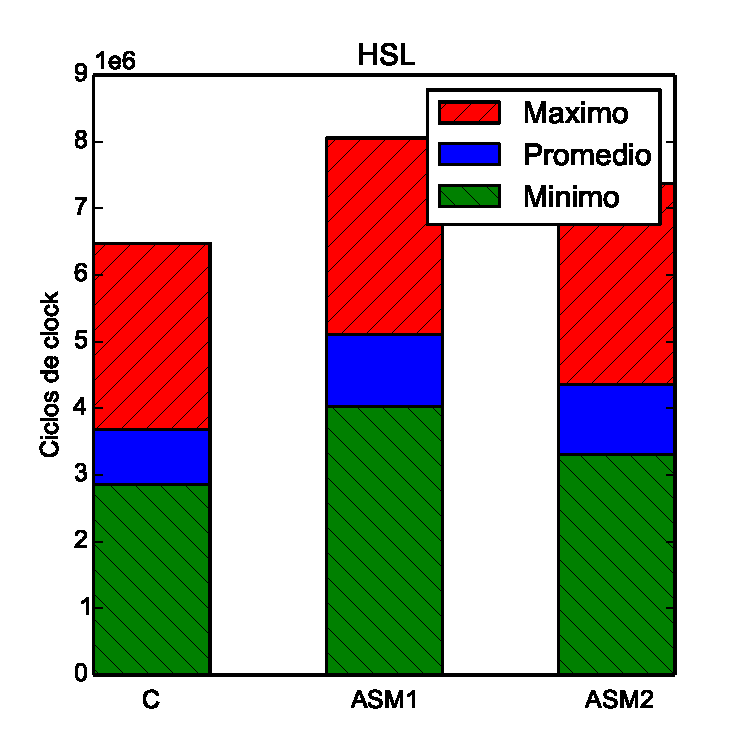
\includegraphics[scale=0.5]{images/hsl_comparation}
\end{figure}

Luego decidimos probar el algoritmo con diferentes imagenes para testear si los saltos condicionales impactan en el rendimiento de las implementaciones.

\begin{figure}[h!]
	\centering
	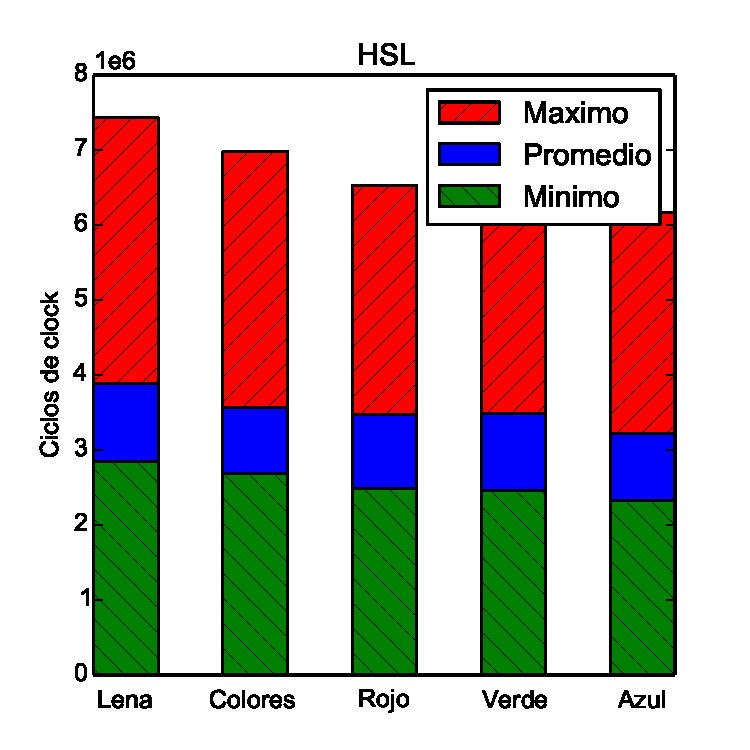
\includegraphics[scale=0.5]{images/hsl_comparationC}
	\caption{C}
	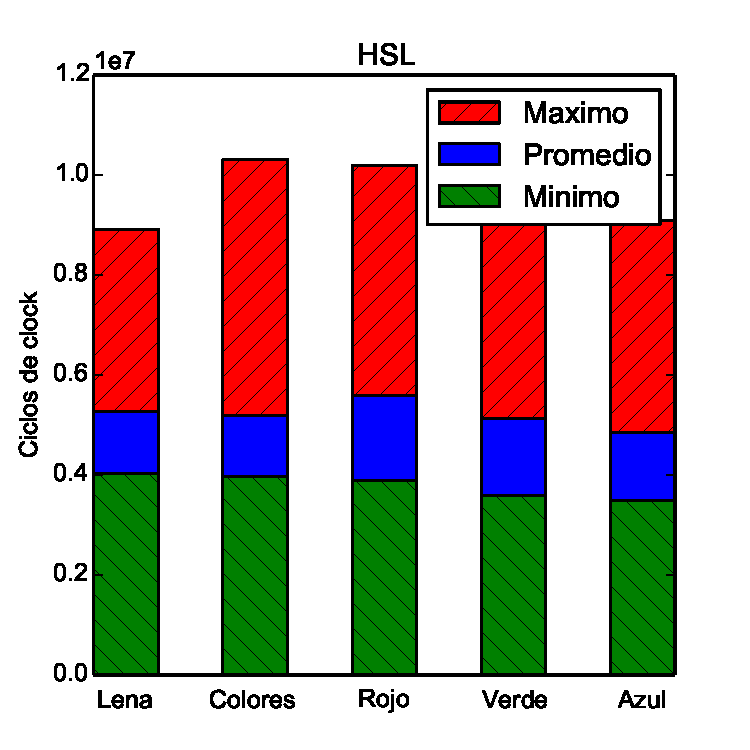
\includegraphics[scale=0.5]{images/hsl_comparationASM1}
	\caption{ASM1}
	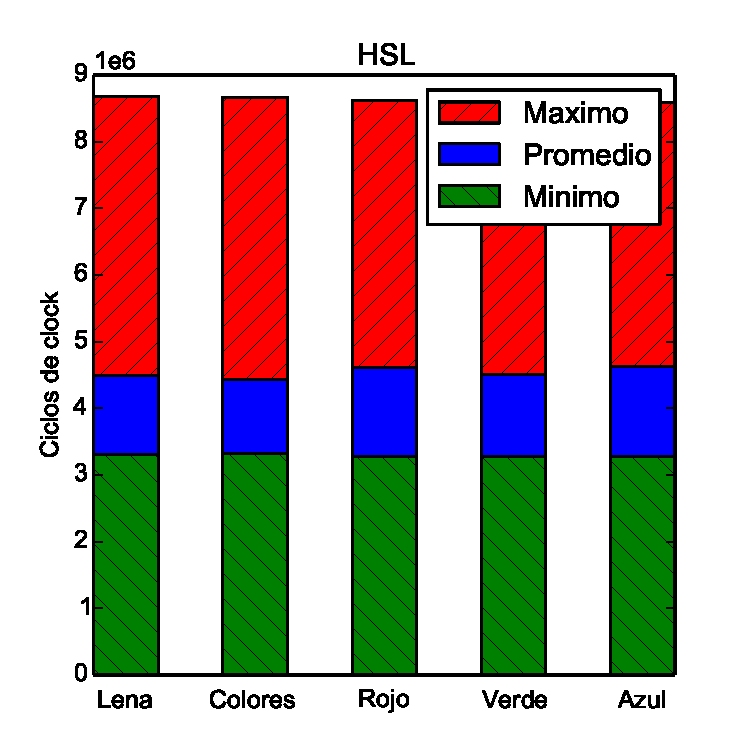
\includegraphics[scale=0.5]{images/hsl_comparationASM2}
	\caption{ASM2}
\end{figure}

\newpage

% Al igual que con los dos casos anteriores, empezamos corriendo la version de $C$ con optimizaciones de nivel 3, junto con la imagen $lena$ brindada por la catedra, se tomaron cien muestras con versiones de la imagen que fuesen multiplos de 16x16, hasta llegar a 320x320. Aqui se encuentran graficados el maximo, minimo y el promedio:\\

% \begin{figure}[h!]
% 	\centering
% 	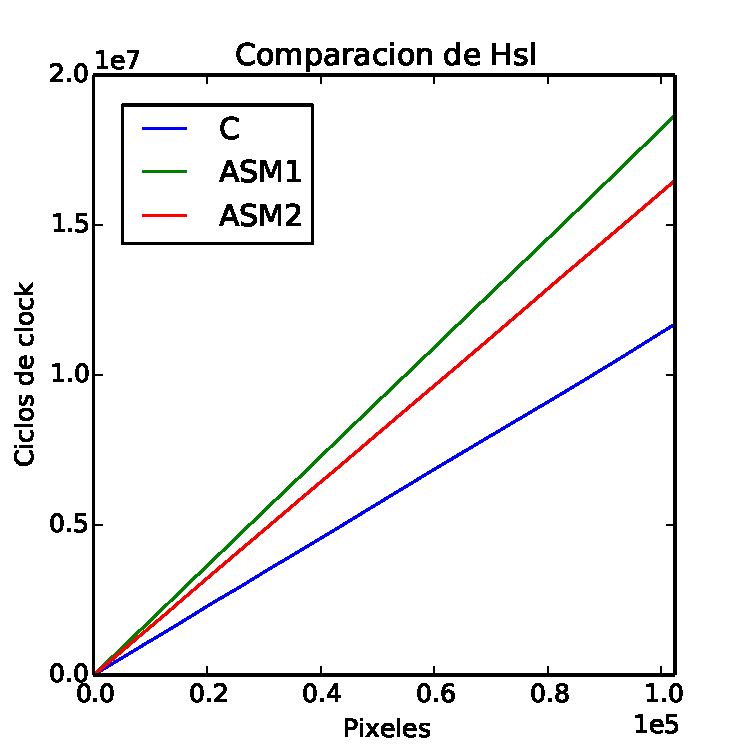
\includegraphics[scale=0.5]{images/c_asm1_asm2_hsl_comp}
% \end{figure}

% Los resultados fueron sorpresivos, ya que a diferencia de los dos filtros anteriores, aqui nos encontramos con que la version de $C$ era mas veloz que las implementaciones de $Assembler$. Esto nos llevo a plantearnos si los saltos condicionales de $C$ , en el peor caso, podian llegar a hacer que las implementaciones en $Assembler$ fuesen mas rapidas. Para probar eso se nos ocurrieron dos tests:\\

% \begin{itemize}
% 	\item Testear imagenes completamente rojas, azules y verdes (una de cada una), junto con $colores$ y $lena$, para ver si el salto condicional en $RGBtoHSL$ impactaba al rendimiento.
% 	\item Testear con diferentes valores de \texttt{HH}, tomando valores aleatorios entre cero y uno para \text{SS} y \texttt{LL}, esto lo hacemos para probar si el condicional de 6 casos en $HSLtoRGB$ afecta el rendimiento.
% \end{itemize}

% Para el primer test se obtuvieron los siguientes resultados:\\

% \begin{figure}[h!]
% 	\centering
% 	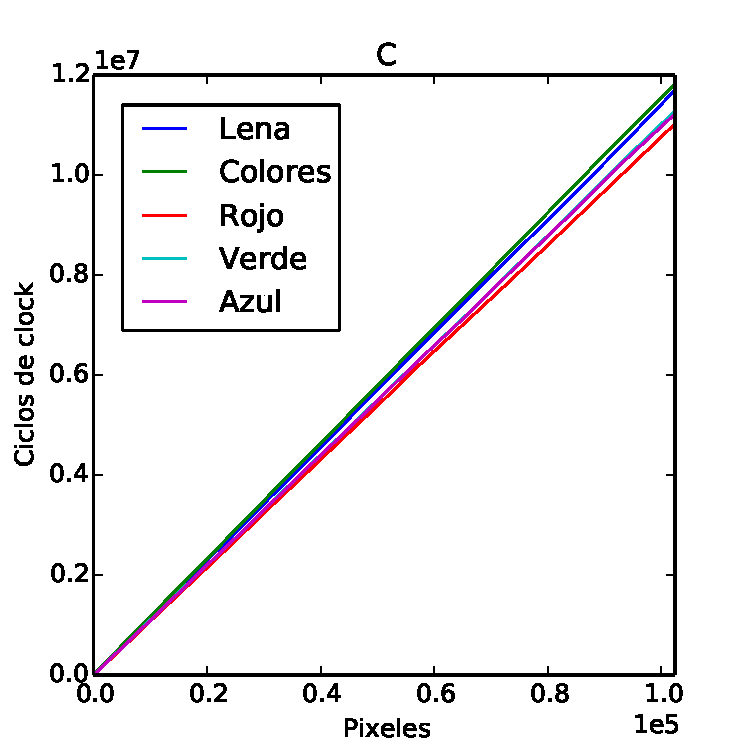
\includegraphics[scale=0.45]{images/c_hsl_lena_colors}
% 	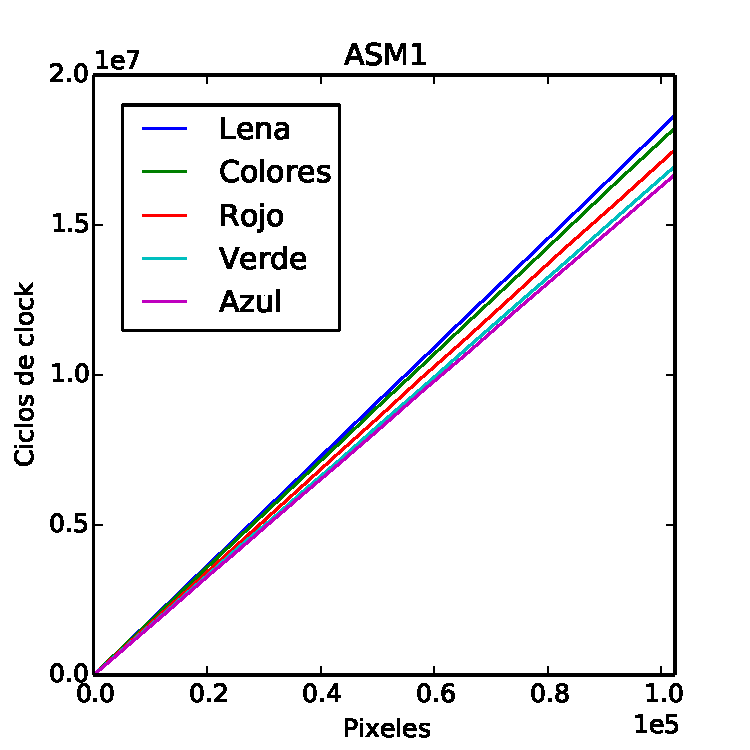
\includegraphics[scale=0.45]{images/asm1_hsl_lena_colors}
% 	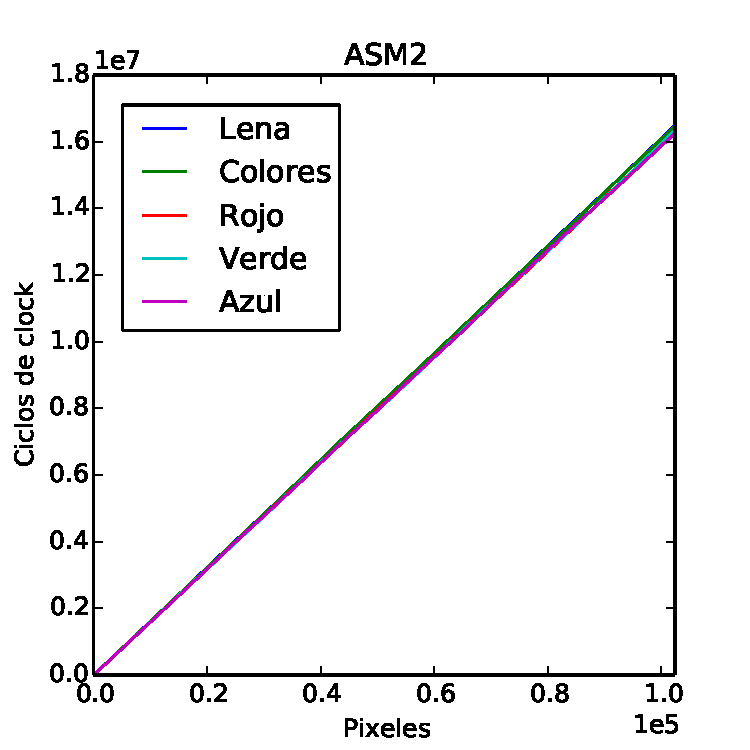
\includegraphics[scale=0.45]{images/asm2_hsl_lena_colors}
% \end{figure}

% Como podemos ver, la segundo implementacion (que no usa ningun tipo de condicional) se matuvo constante independientemente del contenido de la imagen, mientras que la de $C$ y la primer implementacion en $Assembler$, que emplean condicionales tuvieron una diferencia considerable en resultados. De todas formas, la implementacion de $C$ termino siendo la de mejor rendimiento.

% Para el segundo test se obtvieron los siguientes resultados:\\

% \begin{figure}[h!]
% 	\centering
% 	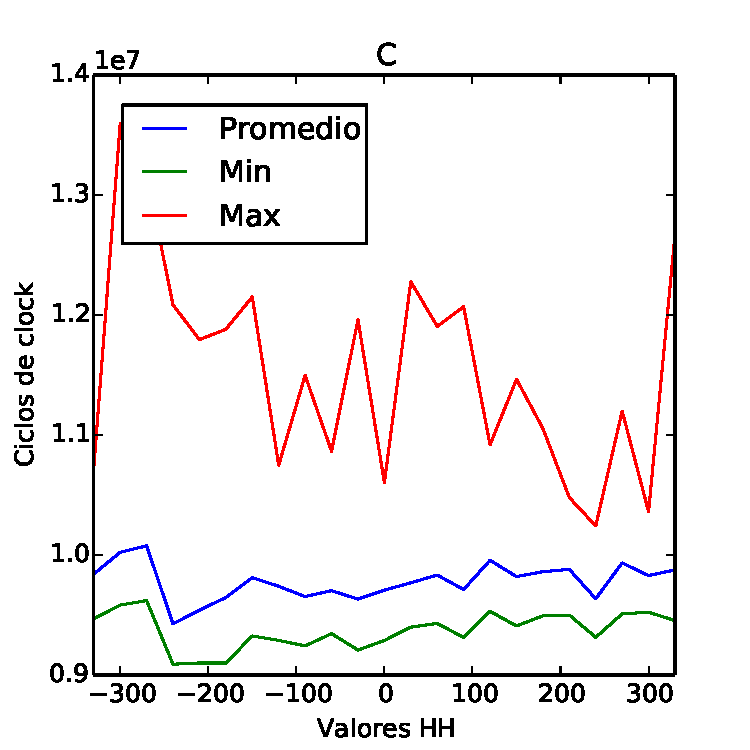
\includegraphics[scale=0.45]{images/c_lenahsl}
% 	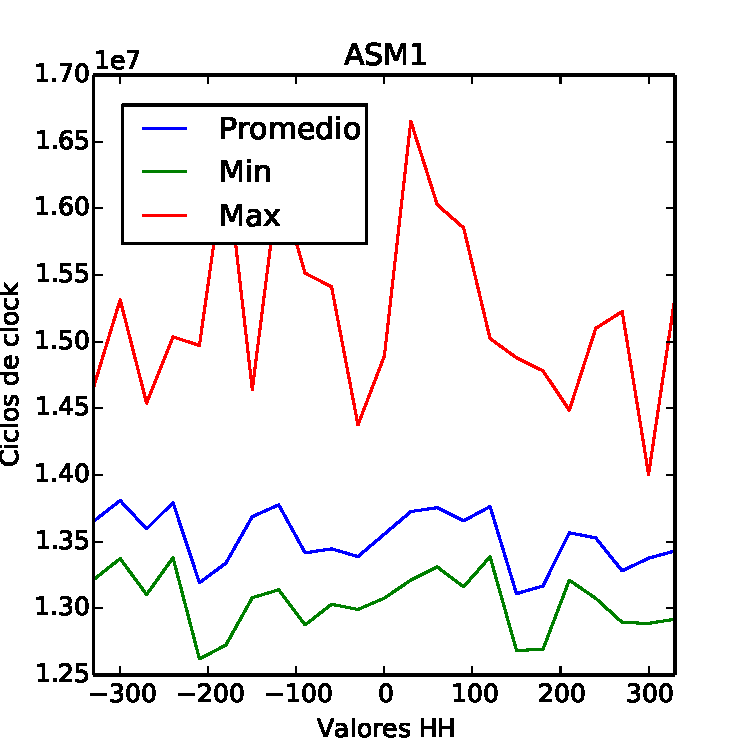
\includegraphics[scale=0.45]{images/asm1_lenahsl}
% 	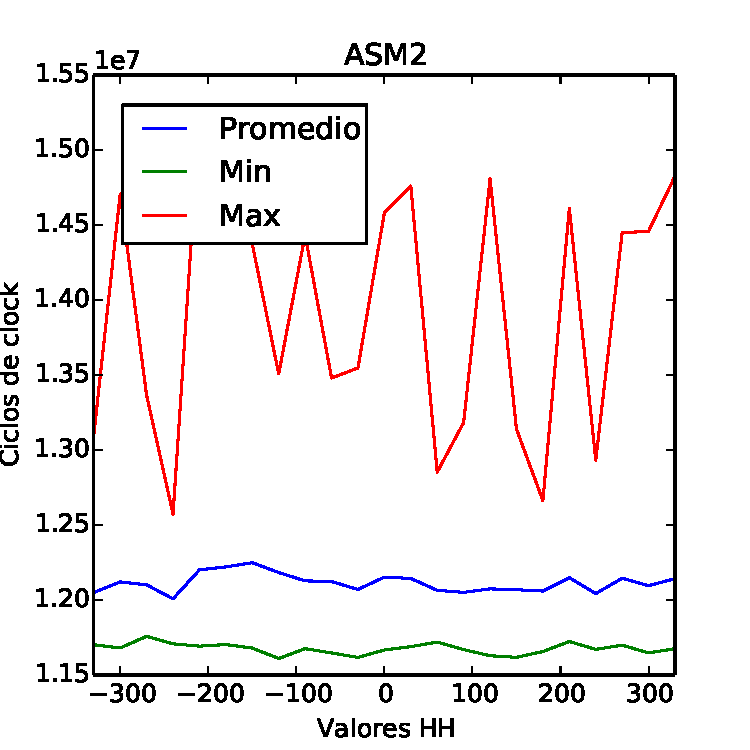
\includegraphics[scale=0.45]{images/asm2_lenahsl}
% \end{figure}

% Aqui podemos ver que el valor de \texttt{HH} no afecta en gran manera al rendimiento, ya que la cantidad de ciclos se mantiene relativamente constante independientemente del \texttt{HH}, y al igual que el primer test, la implementacion de $C$ sigue teniendo mejor rendimiento.

\subsection{Conclusion}
En conclusion podemos ver que la version de C es la mas rapida, suponemos que esto es asi debido a que la prediccion de saltos del procesador es lo suficientemente buena como para que sea mas rapido que hacer las cosas usando SIMD y procesando todo usando mascaras.

Tambien podemos ver tambien que los saltos afectan la consistencia del algoritmo ya que la implementacion ASM2 posee tiempos de ejecucion mucho mas consistentes, en cambio la de C y ASM1 (La cual posee funciones con saltos) poseen variaciones en los tiempos de ejecucion.

% Este filtro trajo varias sorpresas respecto al rendimiento, si bien los condicionales afectaron en mayor o menor medida a la implementacion en $C$, esta termino siendo la mejor en practicamente todos los casos probados. Consideramos que esto se debe a que el trabajo que realiza el filtro no era amigable al paralelismo, es decir, muchas veces se realizaban calculos que luego terminan siendo filtrado por alguna mascara.